\section{Kernel Features}

\begin{frame}{Utility Classes}

\begin{center}
	hhuOS includes some utility classes to ease implementing new features
\end{center}

\vspace{8pt}

\begin{center}
	\begin{tabular}{c c c c}
		\textbf{Array} & \textbf{ArrayList} & \textbf{LinkedList} & \textbf{HashMap}
	\end{tabular}

	\vspace{8pt}
	
	\begin{tabular}{c c c}
		\textbf{HashSet} & \textbf{BlockingQueue} & \textbf{RingBuffer}
	\end{tabular}
\end{center}

\vspace{8pt}

\begin{center}
	Each utility class can be used in conjuction with \\any type by using template parameters
\end{center}

\end{frame}

\begin{frame}{Utility Classes : Arrays}

\begin{center}
	Array copies can be created using a simple assignment
\end{center}

\begin{center}
	\begin{minipage}{0.55\textwidth}
		\begin{codeblock}[code/Arrays.cpp]{C++}
			\cppfile{code/Arrays.cpp}
		\end{codeblock}
	\end{minipage}
	
	\vspace{5pt}
	
	\begin{minipage}{0.22\textwidth}
		\begin{terminalblock}
			\color{termfg}
			\textfile{code/Arrays.term}
		\end{terminalblock}
	\end{minipage}
\end{center}

\end{frame}

\begin{frame}{Utility Classes : HashMaps}

\begin{center}
	HashMaps can be used to store key-value pairs with any type
\end{center}

\begin{center}
	\begin{minipage}{0.79\textwidth}
		\begin{codeblock}[code/HashMaps.cpp]{C++}
			\cppfile{code/HashMaps.cpp}
		\end{codeblock}
	\end{minipage}
	
	\vspace{5pt}
	
	\begin{minipage}{0.41\textwidth}
		\begin{terminalblock}
			\color{termfg}
			\textfile{code/HashMaps.term}
		\end{terminalblock}
	\end{minipage}
\end{center}

\end{frame}

\begin{frame}{Kernel Modules}

\begin{center}
	hhuOS' functionality can be extended using kernel modules
\end{center}

\begin{center}
	\begin{minipage}{\textwidth}
		\begin{codeblock}[code/Hello.h]{C++}
			\cppfile{code/Hello.h}
		\end{codeblock}
	\end{minipage}
\end{center}

\begin{center}
	Each module needs to inherit from the \texttt{Module} class
\end{center}

\end{frame}

\begin{frame}{Kernel Modules}

\begin{center}
	hhuOS's functionality can be extended using kernel modules
\end{center}

\begin{center}
	\begin{minipage}{\textwidth}
		\begin{codeblock}[code/Hello.cpp]{C++}
			\cppfile{code/Hello.cpp}
		\end{codeblock}
	\end{minipage}
\end{center}

\begin{center}
	In this example, the \texttt{Hello} module prints \texttt{Hello hhuOS!} on initialization
\end{center}

\end{frame}

\begin{frame}{Kernel Modules}

	\begin{center}
		hhuOS supports loading kernel modules at runtime
	\end{center}
	
	\begin{center}
		\begin{minipage}{0.725\textwidth}
			\begin{codeblock}[code/Modules.cpp]{C++}
				\cppfile{code/Modules.cpp}
			\end{codeblock}
		\end{minipage}
	
		\begin{minipage}{0.175\textwidth}
			\begin{terminalblock}
				\color{termfg}
				\textfile{code/Modules.term}
			\end{terminalblock}
		\end{minipage}
	\end{center}
	
	\begin{center}
		Compiled modules can be placed on an external storage device
	\end{center}

\end{frame}

\begin{frame}{Bluescreen / Stacktrace}

\begin{center}
	If something goes wrong, hhuOS prints out a bluescreen \\containing useful information such as a stacktrace
\end{center}

\begin{center}
	\begin{minipage}{0.9\textwidth}
		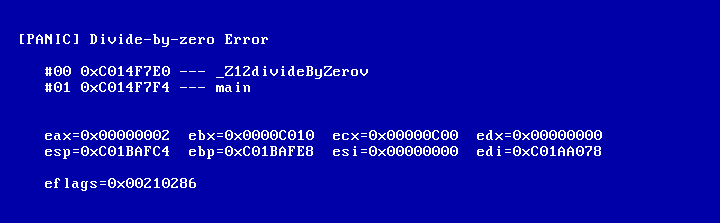
\includegraphics[width=\textwidth]{img/hhuos_bluescreen}
	\end{minipage}
\end{center}

\end{frame}